\newpage
\section{Stato attuale del sistema}
\label{sec:chapter_architettura_sistema_il_servizio}

Questo paragrafo sarà focalizzato sullo stato attuale del sistema. Verrà analizzato nel dettaglio il funzionamento di ognuno dei servizi, visti però come scatole nere; verranno quindi descritte le funzionalità offerte dai servizi mediante le interfaccie da loro esposte.
\\
Come introdotto ad inizio capitolo il sistema è realizzato basandosi su un’architettura di tipo client-server: Questo vuol dire che il sistema è organizzato come:
\begin{itemize}
\item Un insieme di servizi (Editor,Navigator,Baked Service): ciascun servizio è caratterizzato da un’interfaccia basata su un protocollo di richiesta/risposta.
\item Un insieme di server: cioè i componenti che erogano i servizi. Ad ogni servizio può corrispondere un server centralizzato, o più server distribuiti. Nel sistema trattato nel presente elaborato viene utilizzato un server centralizzato che eroga i servizi Editor e Navigator, e un’altro server centralizzato che eroga il Baking Service.
\item Un insieme di client (per client si intende un computer o un browser web): i client sono i componenti fruitori di servizi.
\end{itemize}
Per l’interazione richiesta/risposta tra client e server si usa un connettore, il quale implementa il protocollo di richiesta risposta usato per l’invocazione del servizio.
\\
Adottare uno stile architetturale di questo tipo permette quindi di separare l’applicazione client dai servizi che i client devono usare, e permette di replicare i server per fornire maggiore scalabilità e disponibilità dei servizi. 
\\
Lo sviluppo di un sistema di questo tipo è sostenuto dagli strumenti di Middleware. I middleware sono tecnologie utilizzate per realizzare i connettori, e quindi implementare la comunicazione e le interazioni tra i diversi componenti del sistema distribuito.
\\  
Per concretizzare lo stile architetturale client server è stato necessario individuare il tipo di middleware da realizzare. 
\\
Il vantaggio del middleware è quello di mascherare la necessità di conoscere dettagli implementativi tra servizi comunicanti: questo vuol dire che, nonostante Editor e Baking Service siano realizzati con tecnologie e linguaggi di programmazione differenti, l’Editor può esercitare una richiesta di bake al Baking Service, e quest’ultimo può rispondere all’Editor consegnando il risultato. Il tutto senza che Editor conosca alcun dettaglio del Baking Service.
\\
\begin{figure}[htb]
 \centering
 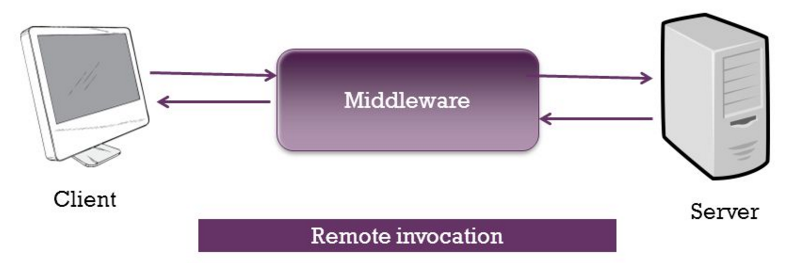
\includegraphics[width=0.8\linewidth]{images/chapter_architettura_sistema/as_middleware.png}\hfill
 \caption[Middleware]{Middleware}
 \label{fig:as_middleware}
\end{figure}
\\
Dopo questa panoramica sul’architettura del sistema verranno mostrate le singole componenti del sistema: funzionalità offerte, input-output scambianti, e interazione con l’utente. 

\section{Servizio Editor}
\label{sec:chapter_architettura_sistema_il_servizio_editor}

L’Editor è normalmente il primo servizio con cui l’utente si interfaccia all’interno del sistema. L’obiettivo è quello di fornire all’utente tutte le funzionalità principali presenti in una applicazione desktop di grafica 3D, ma su un browser web.
\\
L’editor permette la realizzazione di scene 3D con la possibilità, tra le altre, di creare modelli da zero o di importarne gia pronti, di spostarli all'interno della scena nella posizione desiderata e di inserire luci. Una volta terminato il proprio lavoro è possibile salvare in locale il risultato, memorizzandolo in un file JSON contenente tutte le informazioni sulla scena realizzata. Lo stesso file JSON può essere dato nuovamente in input all’editor, per reimportare la scena.
\\ 
Una volta che l’utente ha creato la scena, e ne ha definito un setup di illuminazione, può richiedere un baking delle lightmap della scena, mediante apposita funzione nell’editor.
\\
Nonostante l’editor sia pensato per essere molto semplice da utilizzare, permette comunque all’utente un certo grado di libertà nell’impostare i parametri con cui lanciare determinate funzioni all’interno dell’editor. Tuttavia siccome il servizio di bake viene offerto all’utente in modo che possa fruirne senza proccuparsi di come funziona, non è possibile chiedere di configurare dei parametri che per essere configurati richiederebbero la conoscenza del processo. 
\\
Pertanto è seguita un’attività di studio in cui si è cercato di individuare un unico parametro che potesse essere configurato a mano dall’utente senza però dover conoscere nulla del processo in cui viene impiegato. La scelta è ricaduta su un parametro detto \emph{sampling}; impostandolo a valori alti, il risultato è un bake di migliore qualità, ma dal processamento più lungo; al contrario un sampling basso indica minore qualità, ma un processamento più rapido. Quindi l’utente che vuole effettutare il bake della sua scena, deve configurare i parametri di bake che saranno il sampling, un nome arbitrario da dare alla scena, e un indirizzo email.
\\
A questo punto, in modo trasparente all’utente, l’editor si occupa di memorizzare la scena nel formato di interscambio dei dati mostrato nel paragrafo \ref{sec:chapter_architettura_sistema_formato_scambio} e di inviare una richiesta HTTP, comprendente scena e parametri di configurazione del bake, al servizio remoto di baking. Per inviare grandi quantità di dati il metodo della richiesta deve essere \texttt{POST}.
\\
Durante il bake l’utente può decidere attraverso l’editor di monitorare lo stato del processo, per sapere a che percentuale di completamento si trova, ed eventualmente può decidere di annullarlo. 
\\
Dal momento che l’esecuzione del bake avviene in remoto su un calcolatore diverso da quello dove gira il client, la disponibilità dell’editor rimane invariata; questo vuol dire che l’utente può continuare ad utilizzare il servizio senza problemi, ed eventualmente può fare richiesta di ulteriori bake. 
\\
Il supporto alla disponibilità da parte dell’editor è inoltre ottenuto dal fatto che in caso di fallimento (ad esempio un’interruzione della linea, on un calo di corrente), per quanto riguarda il bake non c’è alcuna perdita di dati all’indietro. Questo perchè il processo sta girando in remoto su un’altro calcolatore, e quindi non solo non verrà perso il risultato, ma al ripristino del fallimento sarà possibile continuare a monitorare lo stato del, o dei processi di bake richiesti.
\\
Una volta che il bake è terminato l’utente riceverà un’email dove verrà notificato l’esito positivo del bake e un link dal quale poter scaricare il risultato; in caso di errore l’email notificherà il fallimento. 
\\
Il risultato consiste in un file JSON descritto mediante lo stesso standard usato dall’editor per l’inviare la scena al servizio di bake. Il file contiene la scena 3D creata dall’utente insieme a tutte le informazioni computate dal processo di baking.
\\
A questo punto l’utente ha la possibilità di reimportare la scena nell’editor, qualora volesse apportare dei miglioramenti a mano, oppure può fruirla mediante il servizio Navigator.
\\
\begin{figure}[htb]
 \centering
 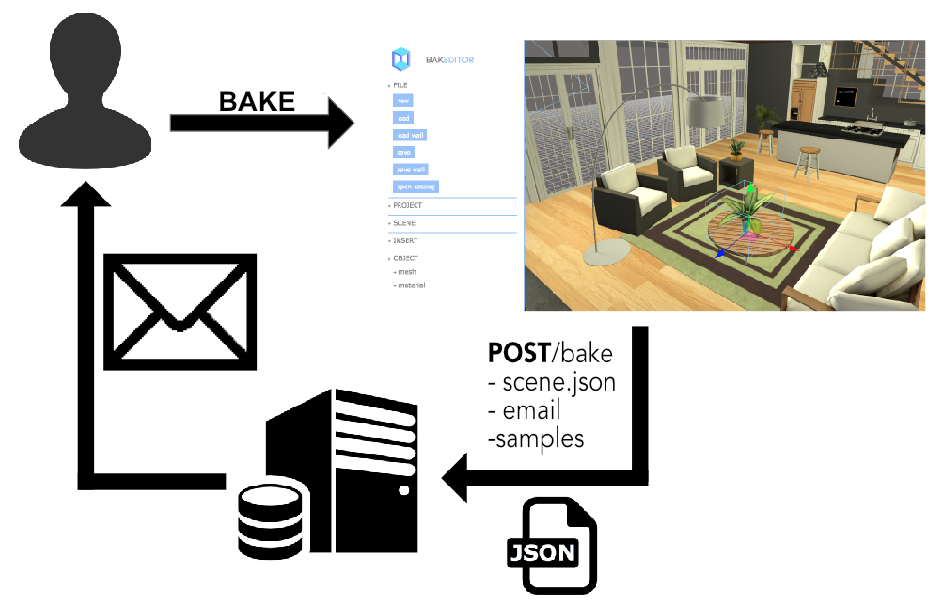
\includegraphics[width=0.8\linewidth]{images/chapter_architettura_sistema/as_editor.png}\hfill
 \caption[Schema architetturale editor]{Schema architetturale dell'editor}
 \label{fig:as_editor}
\end{figure}
\\
L'editor è stato realizzato utilizzando la libreria Javascript Three.js ed organizzato seguendo la filosofia delle tecnologie Web Components mediante il framework Polymer.
\section{Servizio Navigator}
\label{sec:chapter_architettura_sistema_il_servizio_navigator}

Il Navigator offre all’utente l’esperienza di navigare in prima persona un’ambiente fotorealistico virtuale.
\\
Anche in questo caso il servizio è fruibile come applicazione web tramite browser, e non richiede quindi alcuna attività di installazione o aggiornamento.
\\
Come già visto nel paragrafo precedente, una volta effettuato il bake la scena è subito fruibile dall’utente; questo vuol dire il Navigator dovrà garantire un livello di qualità nella navigazione che sia indipendente dal tipo di scena fruita dall’utente.
\\
Sono gia presenti sul mercato web delle applicazioni che consentono di navigare un’interno fotorealistico creato dall’utente, ma sia la creazione che la navigazione sono supervisionati. Questo vuol dire che una volta realizzata la scena, questa non sarà immediatamente fruibile dall’utente, ma dovrà passare per una fase di processamento dove verrà configurata un’esperienza di navigazione ad hoc per il tipo di ambiente.
\\
La necessità di realizzare un navigatore che funzionasse indipendentemente dal tipo di scena, ha richiesto lunga attività di studio e sperimentazioni per garantire tutte quelle qualità tipiche di una navigazione in prima persona, come la gestione delle collisioni, o la possibilità di salire o scendere le scale. 
\\
Il navigator è scalabile sulla stragrande maggioranza delle piattaforne hardware; questo perchè la pipeline di rendering processata durante la navigazione dell’utente è la versione lightweight, mostrata nel capitolo \ref{cha:chapter_lrl}. 
\\
Nel paragrafo si è discusso infatti come nella scena realizzata dall’utente non ci siano luci, ombre, riflessioni, o rifrazioni da calcolare. Nonostante il lightweight render loop diminuisca il carico di lavoro da parte dell’hardware grafico del client, alcune funzionalità come la gestione delle collissioni potrebbero gravare a livello di prestazioni sulla CPU. 
\\
Per far si che le prestazioni del navigator si adattino a fronte di un carico simile, è stato necessario ottimizzare le funzionalità del navigator più onerose dal punto di vista computazionale.
\\
Il Navigator permette la fruizione della scena mediante diverse modalità di navigazione:
La prima modalità, che poi è quella di default, permette di osservare la scena dall’alto, e di interagire con essa muovendola o zoomando su di essa. Come gia discusso nel paragrafo \ref{sec:chapter_stato_arte_rendering_pipeline}  sarà compito dello stadio Applicazione tradurre azioni come uno slide laterale con il cursore del mouse, o un pinch out con le dita, in una rotazione o uno zoom sulla scena.
\\
La seconda modalità, e probabilmente quella più importante, permette all’utente di navigare la scena in prima persona. Gran parte dello sviluppo del servizio Navigator è stato dedicato alla realizzazione di questa modalità; il motivo è la già accennata necessità di implementare funzionalità come il calcolo delle collisioni, non necessario nella prima modalità, cercando di ottimizzarle a causa della mole di lavoro aggiuntvo richiesto all’hardware sottostante.
\\
La terza e ultima modalità sfrutta la possibiità di far girare il Navigator su sistemi mobile; questa caratteristica è abilitante per l’utilizzo di tecnologie come i visori per la realtà virtuale. Questi visori sono una tecnologia a buon mercato, e permettono di utilizzare lo smartphone come mezzo per annulare la realtà dalla visuale dell’utente. Mediante apposità modalità nel Navigator è quindi possibile navigare la scena in prima persona utilizzando un visore per la realtà virtuale, vivendo così un’esperienza molto più realistica. 
\\
Per quanto riguarda l’interazione con l’utente, il Navigator è un servizio molto semplice da utilizzare: una volta scaricata la scena dal link indicato nell’email inviata dal Baking Service, è sufficiente accedere al servizio Navigator mediante apposita URL. A questo punto l’utente importa la scena nel navigator e sceglie la modalità di navigazione che preferisce. In qualsiasi momento l’utente può scegliere di cambiare modalità, rimuovere la scena o importarne una nuova.
\\
\begin{figure}[htb]
 \centering
 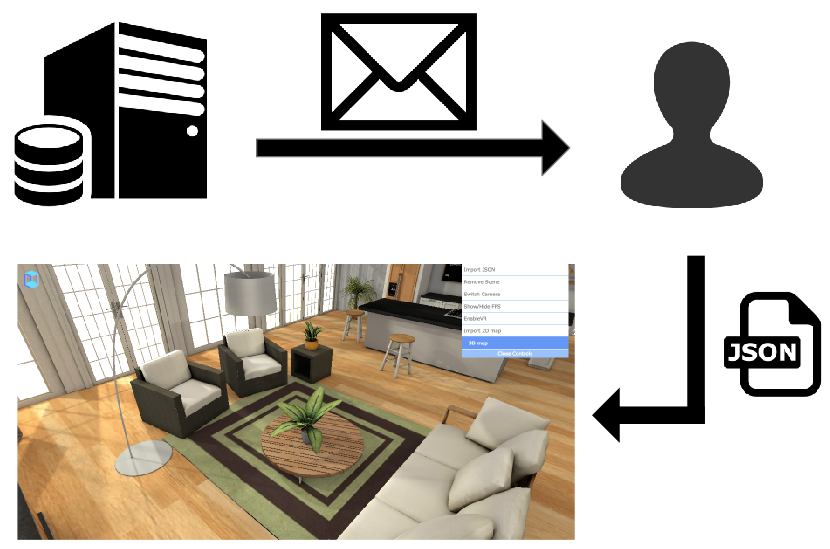
\includegraphics[width=0.8\linewidth]{images/chapter_architettura_sistema/as_navigator.png}\hfill
 \caption[Schema architetturale navigator]{Schema architetturale del navigator}
 \label{fig:as_navigator}
\end{figure}

\section{Servizio di Bake}
\label{sec:chapter_architettura_sistema_il_servizio_baking}

Nella sezione dedicata all’editor si è fatto cenno a come il servizio dia all’utente la possibilità di invocare l’esecuzione di un bake, e come in modo trasparente all’utente l’editor traduca questa invocazione in una richiesta ad un server remoto. Su questo server è installato il servizio di bake. 
\\
Tale servizio è una applicazione web lato server che si impegna ad ascoltare le richieste del client, e ad invocare i processi corrispondenti. 
\\
Per far sì che il servizio Editor sul client possa fare una richiesta da remoto al Baked Service, deve essere possibile un’interazione richiesta/risposta tra client e server.
\\ 
Il Baked Service può essere visto in modo astratto come una funzione che prende in input una richiesta, e in output produce una risposta.
\\ 
Il problema che la funzione deve risolvere è quello di effettuare il bake delle lightmap della scena fornita in input con la richiesta, e produrre in output una risposta con la scena elaborata. Tuttavia questa non è l’unica operazione che viene effettuata. 
\\
Siccome il servizio opera in ambiente web, prima di effettuare l’operazione di bake sono necessari una serie di pre e post processamenti:
Per prima cosa i parametri di bake allegati nella richiesta insieme alla scena devono essere validati, nell’eventualità che ci siano errori. 
\\
Dopodichè bisogna memorizzare l’input, ovvero la scena allegata nella richiesta.
\\ 
Siccome in ambiente web vi è la possibilità che le richieste di bake provengano da utenti multipli, è di fondamentale importanza gestire una coda delle richieste. Seguendo l’ordine previsto dalla coda le richieste sono elaborate, chiedendo a Blender, che è installato sulla macchina che opera da server, di processare il baking delle lightmap sulla scena precedentemente memorizzata.
\\ 
Una volta terminato il baking viene spedita la mail all’utente, con l’esito del bake da lui richiesto. 
\\
Come è possibile notare, il problema che la funzione di baking deve risolvere può essere decomposto in una lunga trama di sottoproblemi. Implementare soluzioni autocontenute ad ognuno di questi sottoproblemi risulta un approccio nettamente più efficiente.
\\
La funzione Baking Service può essere quindi organizzata come un’insieme di funzioni più piccole; 
le richieste dell’utente verranno dunque processate da una decomposizione di passi di elaborazione successivi, detta pipeline di elaborazione. 
\\
Condizione abilitante affinchè il server invochi la pipeline di elaborazione sopra citata è la ricezione di una richiesta di bake da parte del client.
\\ 
Il sistema descritto nel presente lavoro di tesi prevede che le richieste che possono essere sottomesse al servizio di bake da parte del client siano molteplici, e ad ognuna corrisponde una successione di passi di elaborazione diversa.
\\ 
E’ importante che il server venga istruito sulle richieste per le quali è prevista l’esecuzione di una pipeline di elaborazione; questo è possibile configurando una tabella routing per il server. Questa procedura è molto importante, in funzione del fatto che le richieste sottomesse dall’utente possono non essere esclusivamente richieste di bake. 
\\
Ad esempio, a fronte di una richiesta di bake, l’utente ha la possibiltà, sempre tramite Editor, di chiedere lo stato di completamento del processo. Questa richiesta di status è completamente diversa dalla richiesta bake, quindi il server deve poterle diversificare e invocare i processi corrispondenti. Quanto affrontato in questa sezione è solo una descrizione generale sul comportamento del sistema. Nel capitolo \ref{cha:chapter_baking_service} verrà descritto nel dettaglio il servizio di baking.